\documentclass[11pt,letter, swedish, english
]{article}
\pdfoutput=1

\usepackage{../custom_as}

\usepackage{listings} 
\usepackage[framed,numbered,autolinebreaks,useliterate]{../mcode}
\lstloadlanguages{matlab} 
\lstset{language=matlab} 

\usepackage[makeroom]{cancel}
\graphicspath{{figures/}}


\swapcommands{\Omega}{\varOmega}

%%Drar in tabell och figurtexter
%\usepackage[margin=10 pt]{caption}
%%För att lägga in 'att göra'-noteringar i texten
\usepackage{todonotes} %\todo{...}

%%För att själv bestämma marginalerna. 
\usepackage{geometry}

%%För att ändra hur rubrikerna ska formateras


%\renewcommand{\thefootnote}{\fnsymbol{footnote}}

\renewcommand{\thesubsection}{\arabic{section} (\alph{subsection})}
\renewcommand{\thesubsubsection}{\arabic{section} (\alph{subsection},\,\roman{subsubsection})}

\newcommand{\Dx}{\ensuremath{\Delta{x}}}
\newcommand{\Dt}{\ensuremath{\Delta{t}}}

\begin{document}




%%%%%%%%%%%%%%%%% vvv Inbyggd titelsida vvv %%%%%%%%%%%%%%%%%

\title{Numerical solutions to PDE's -- AMATH\,741 \\
Assignment 3}
\author{Andréas Sundström}
\date{\today}

\maketitle

%%%%%%%%%%%%%%%%% ^^^ Inbyggd titelsida ^^^ %%%%%%%%%%%%%%%%%

\section{Numerical investigation of numerical dissipation and dispersion}
In this problem we will be dealing with numerical schemes of the form
\begin{equation}
U_j^{n+1}=(1-\beta)U_j^n+\frac{\beta-\alpha}{2}U_{j+1}^n+\frac{\alpha+\beta}{2}U_{j-1}^n
\end{equation}
for solving the linear advection equation $u_t+au_x=0$. Here
$\alpha=a\Dt/\Dx$ and $\beta$ depends on the scheme:
\begin{center}
\begin{tabular}{l|c|c|c|c|}\cline{2-5}
& Upwind & Lax-Friedrichs & Lax-Wendroff & Centered\\ \hline
\multicolumn{1}{|l|}{$\beta$: }&$|\alpha|$&$1$&$\alpha^2$&0\\ \hline
\end{tabular}
\end{center}

It is easy to show that, with \emph{periodic boundary conditions},
each time step can be represented using a transfer matrix,
$U^{n+1}=\mathsf{T}U^n$ where
\begin{equation}
\mathsf{T}=\begin{bmatrix}
D_0&D_{+1}&0&\cdots&0&0&D_{-1}\\
D_{-1}&D_0&D_{+1}&0&\cdots&0&0\\
0&D_{-1}&D_0&D_{+1}&0&\cdots&0\\
\vdots&&&\ddots&&&\vdots\\
0&\cdots&0&D_{-1}&D_0&D_{+1}&0\\
0&0&\cdots&0&D_{-1}&D_0&D_{+1}\\
D_{+1}&0&0&\cdots&0&D_{-1}&D_0\\
\end{bmatrix}
\end{equation}
and $D_0=(1-\beta)$, $D_{-1}=(\alpha+\beta)/2$ and
$D_{+1}=(\beta-\alpha)/2$. 
This is them implemented in MATLAB through:
\lstinputlisting{code/spTranferMatrix.m}

With the matrix, the rest is just a matter of looping through all time
steps. That is if we want to know how the solution looks at each time
step. But we're only interested in the solution after a certain number
of time steps, $N$, so all we have to do is to calculate
\begin{equation}
U^{N}=\mathsf{T}^NU^{0}.
\end{equation}
I have also listed all the relevant numerical parameters I've used in
each part of this problem in \tabref{tab:1_num_par}.

The initial condition used in the first three parts is just $u(x,
0)=\sin(6\pi x)$, and in 1d $u(x, 0)=\exp(-x^2/0.02)$ was used. The
exact solution would just be the function shifting without any change
in amplitude. 

\begin{table}\centering
\caption{Table of all the relevant numerical parameters used in each
  part of this problem. The IC of $u(x, 0)=\sin(6\pi x)$ was used in
  all parts, but 1d where $u(x, 0)=\exp(-x^2/0.02)$ was used. }
\label{tab:1_num_par}
\begin{tabular}{l|c|c|c|c|c|c|}\cline{2-7}
& $\Dx\times10^3$ & $\alpha$ 
& $\Dt\times10^3$ & $N$& $t_N$ & Scheme
\\ \hline
\multicolumn{1}{|l|}{1a} 
& 4, 14, 20 & 0.6 & 2.4, 8.6, 12 
& 4166, 1162, 833 & 10 & LW
\\ \hline
\multicolumn{1}{|l|}{1b} 
& 20 & 0.6 & 12 & 833 & 10 & ---
\\ \hline 
\multicolumn{1}{|l|}{1c} 
& 4 & 0.1, 0.5 0.9 & 0.4, 2.0, 3.6
& 1250, 250, 138 & 0.5 & LF
\\ \hline
\multicolumn{1}{|l|}{1d} 
& 20 & 0.6 & 12 
& 849 & 10.2 & LW
\\ \hline
\end{tabular}
\end{table}

The results for part a through d will just be presented in figures 1
through 4 and their captions.

\newgeometry{top=1cm, bottom=3cm}
%\subsection{Numerical dissipation depending on $\Dx$}
\begin{figure}
\centering
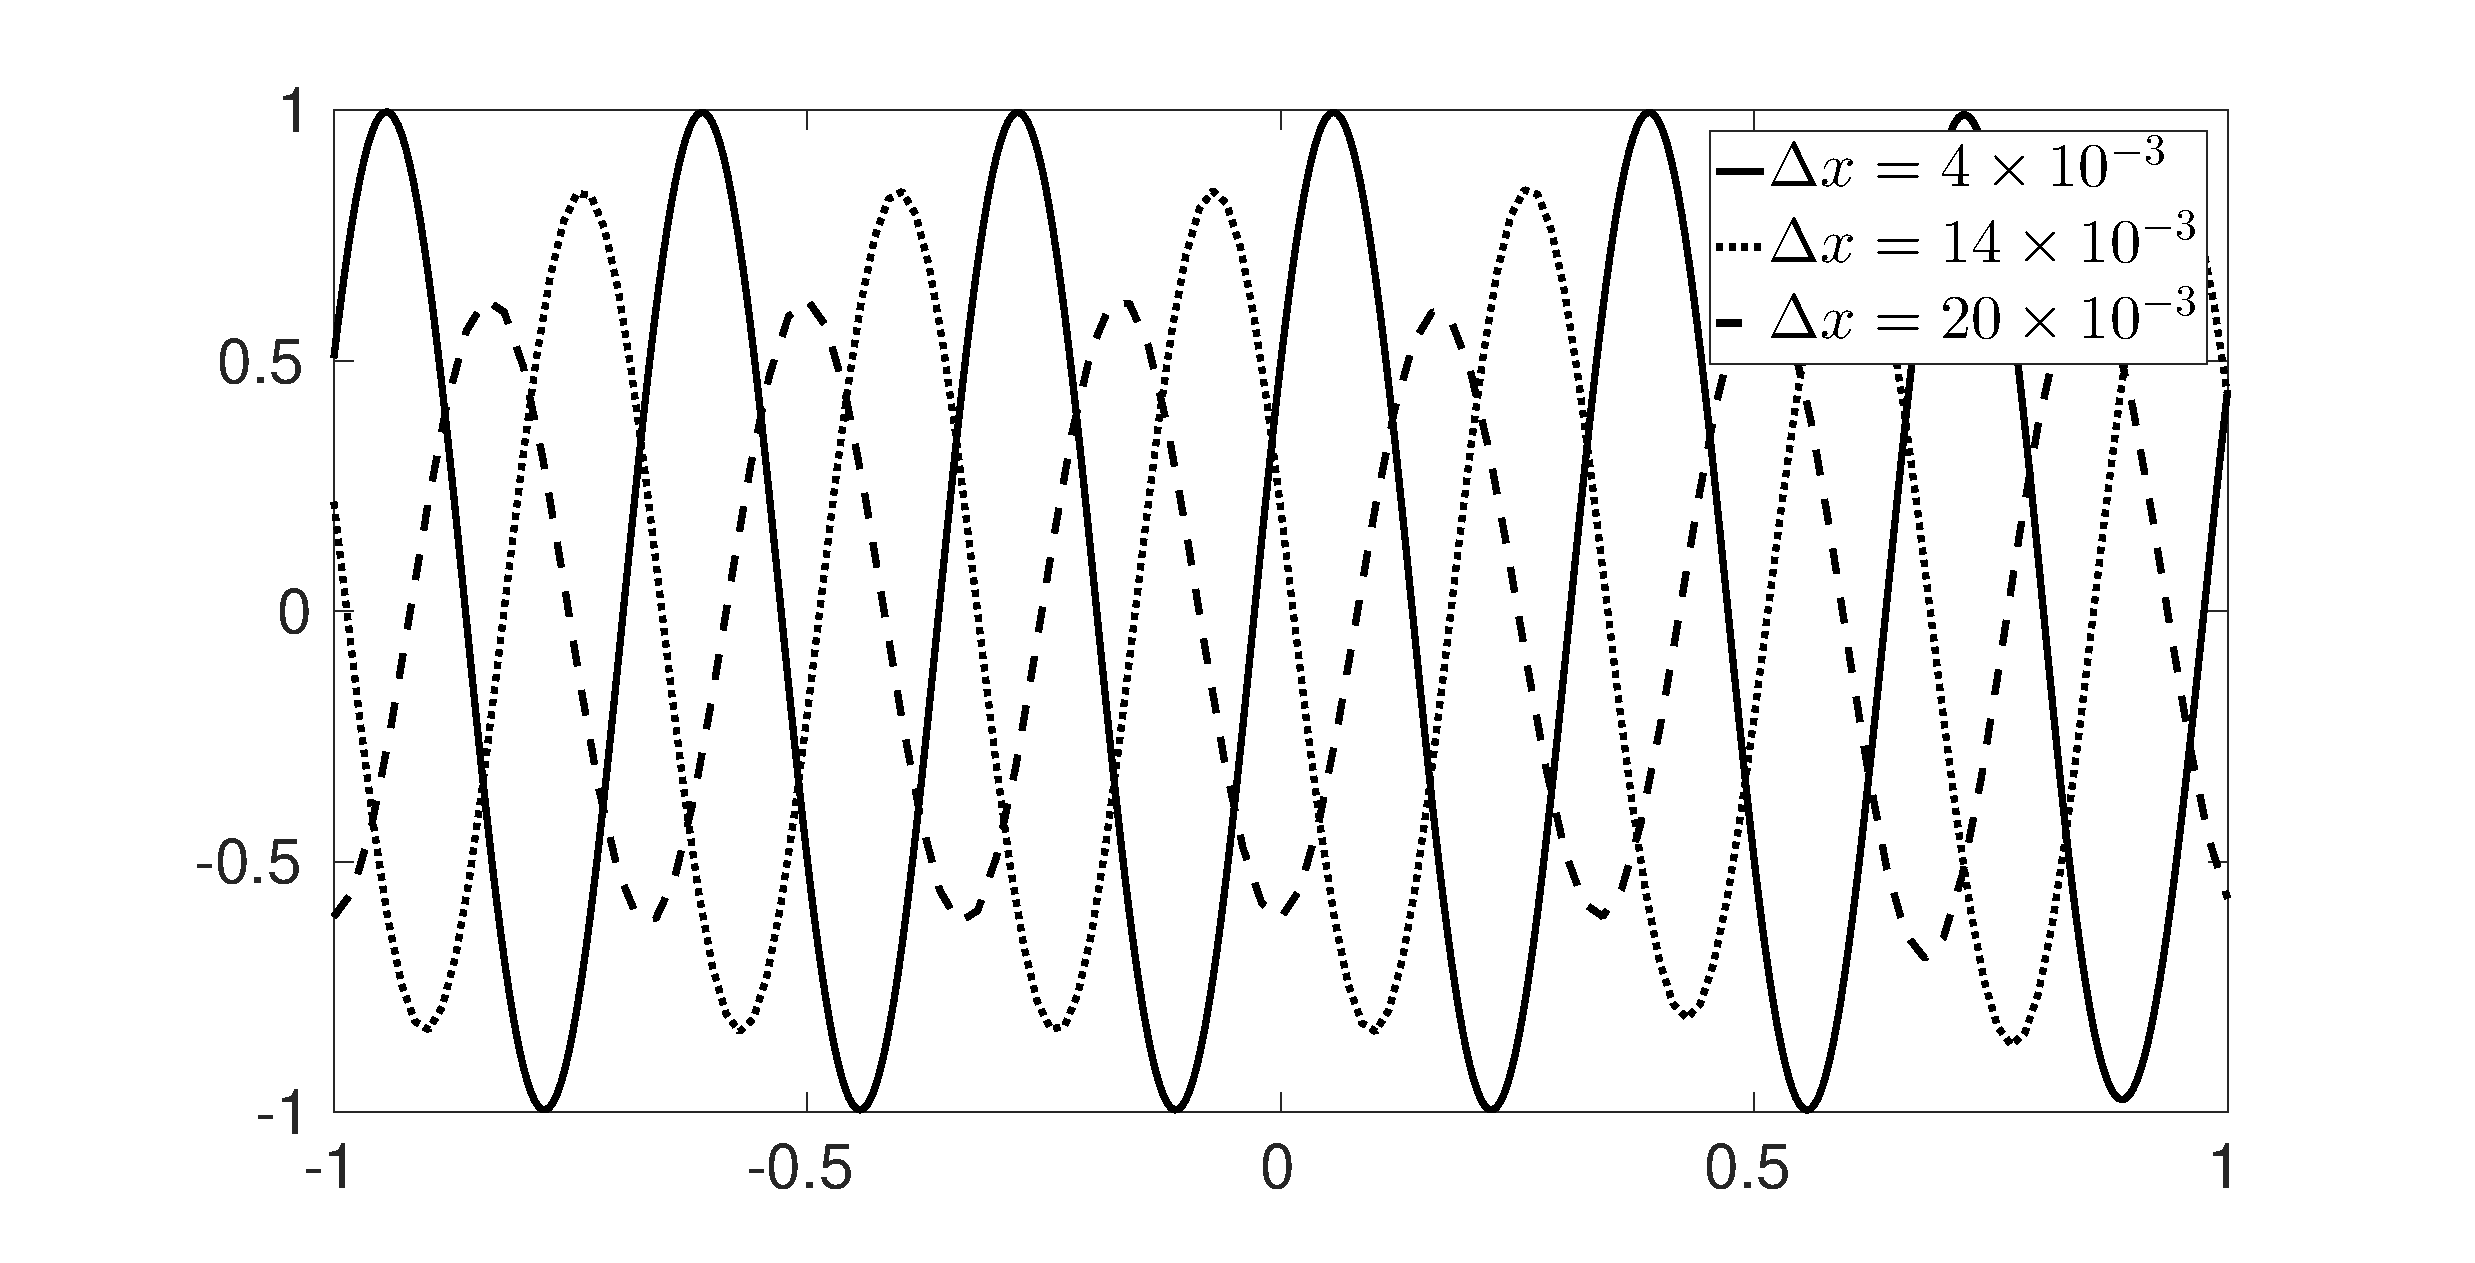
\includegraphics[width=1\textwidth]{1a.eps}
\caption{(1a) The effects of different $\Dx$ on the numerical
  dissipation. The plot is of numerical solutions, using LW, of the
  advection equation, but with different mesh sizes. We can clearly
  see that the larger we choose $\Dx$, the more numerical dissipation
  we get. We can also observe different rates of dispersion, but more
  on that later. }
\label{fig:1a}
\end{figure}

%\subsection{Numerical dissipation depending on scheme}
\begin{figure}
\centering
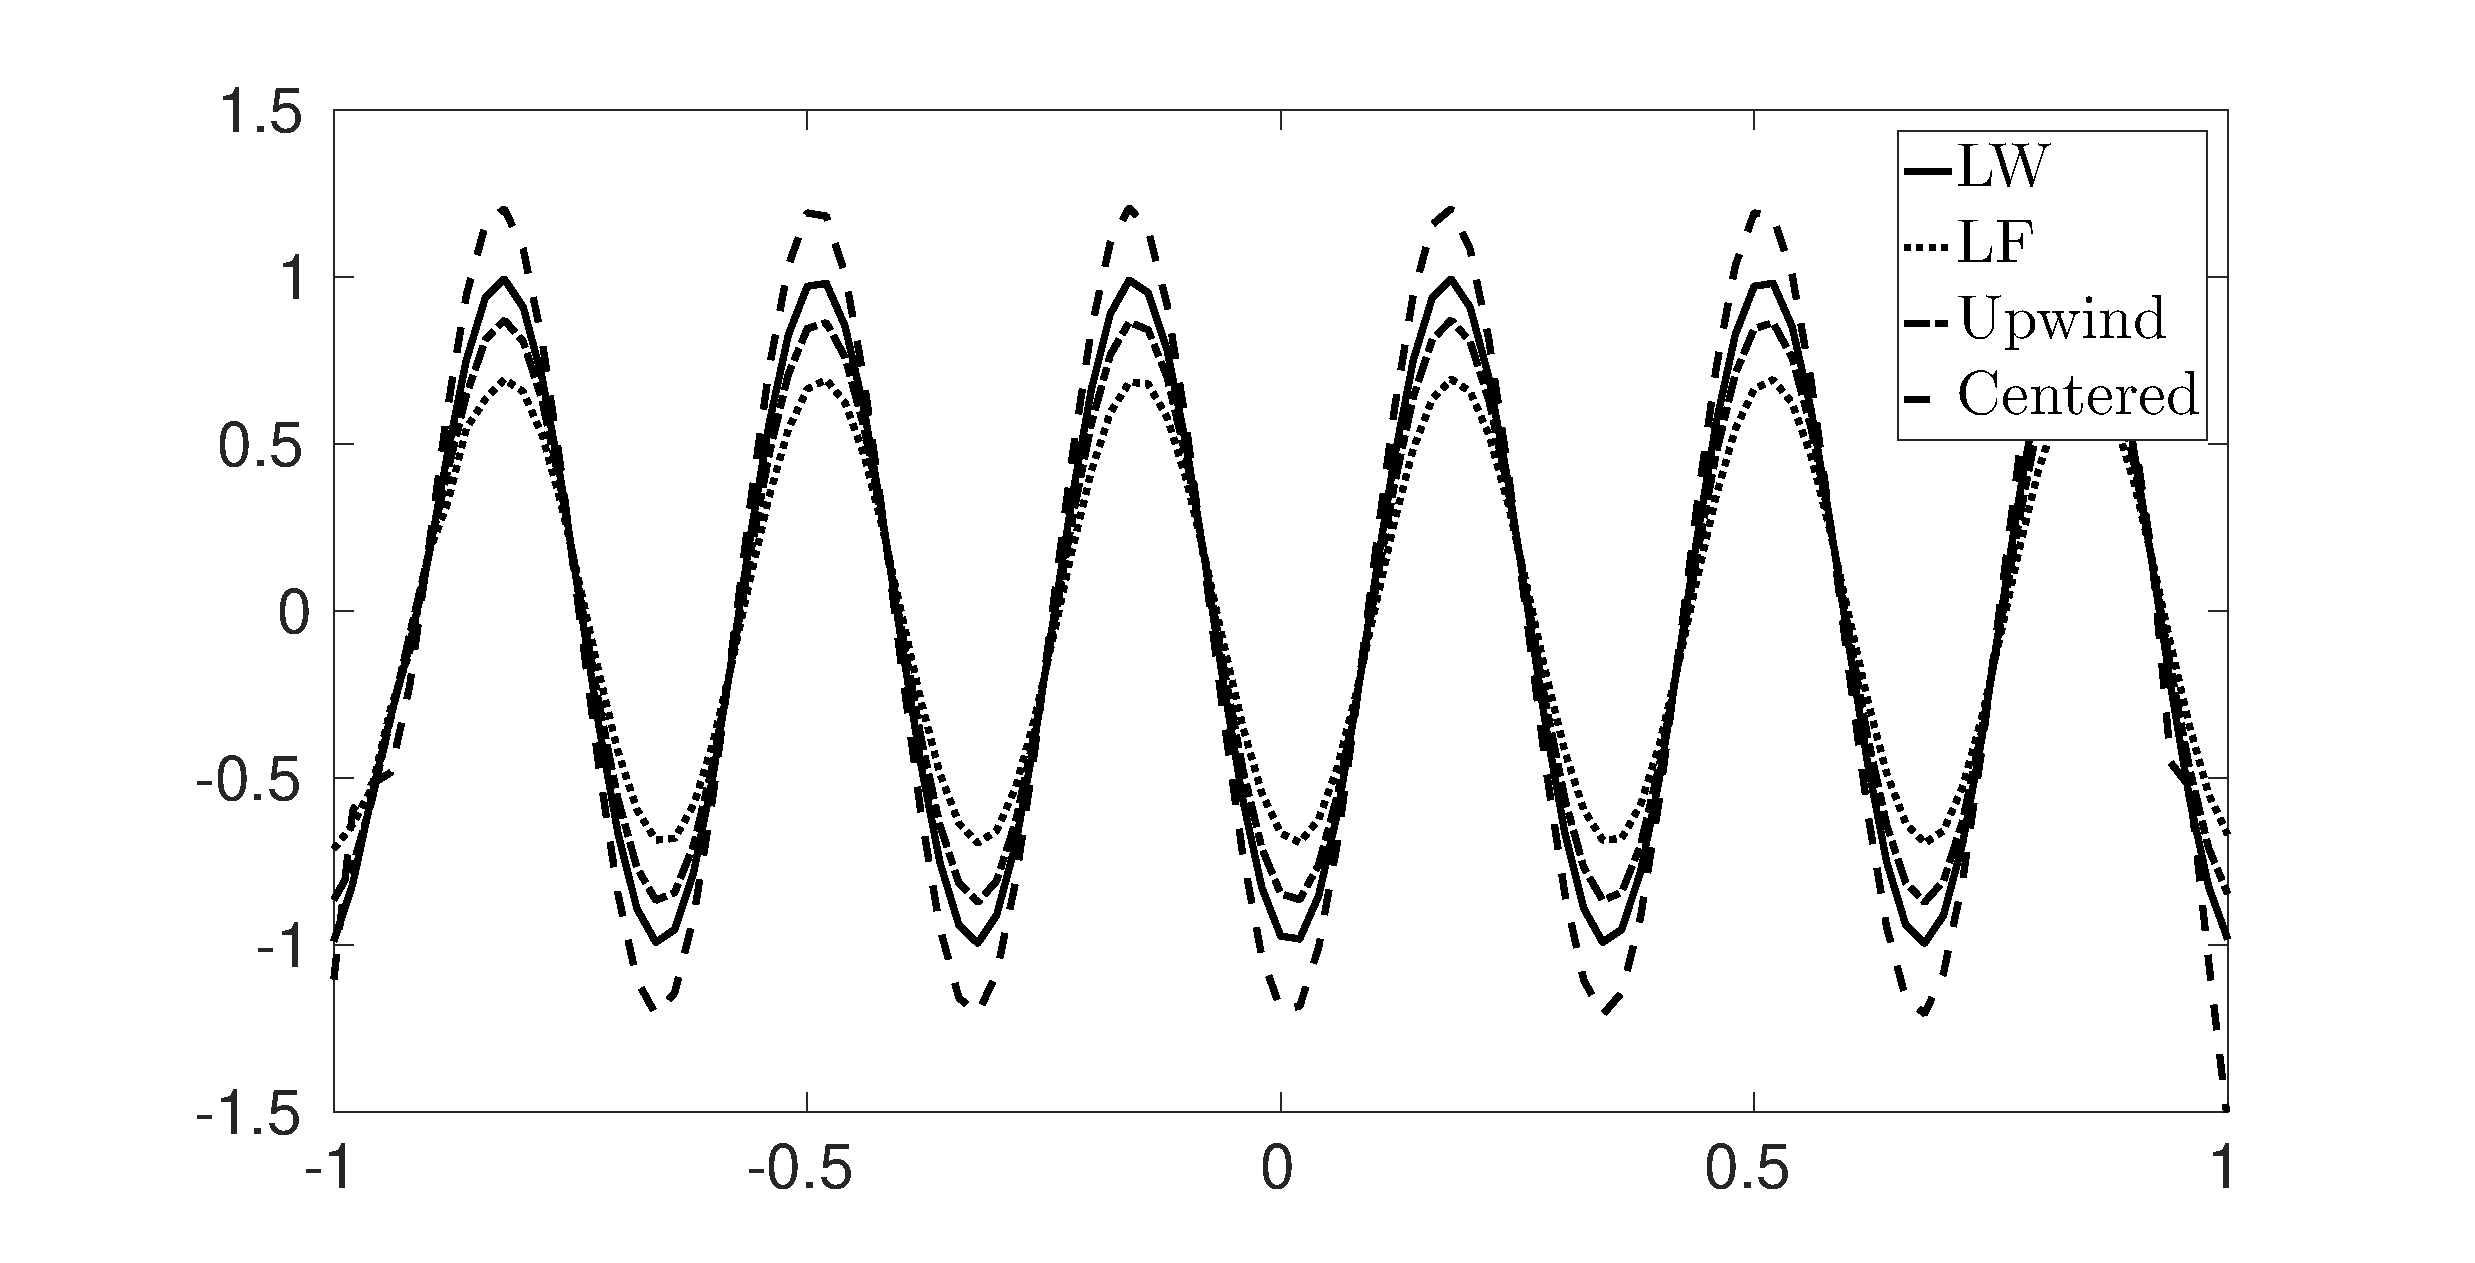
\includegraphics[width=1\textwidth]{1b.eps}
\caption{(1b) Result from different numerical schemes. We can begin by
noting that LW is closest to the original amplitude of 1, where as the
other schemes have resulted in amplitude change. Also notable is that
the centered scheme resulted in an increasing amplitude, which is
generally unwanted. }
\label{fig:1b}
\end{figure}


%\subsection{The affects of the size of $\Dt$}
\begin{figure}
\centering
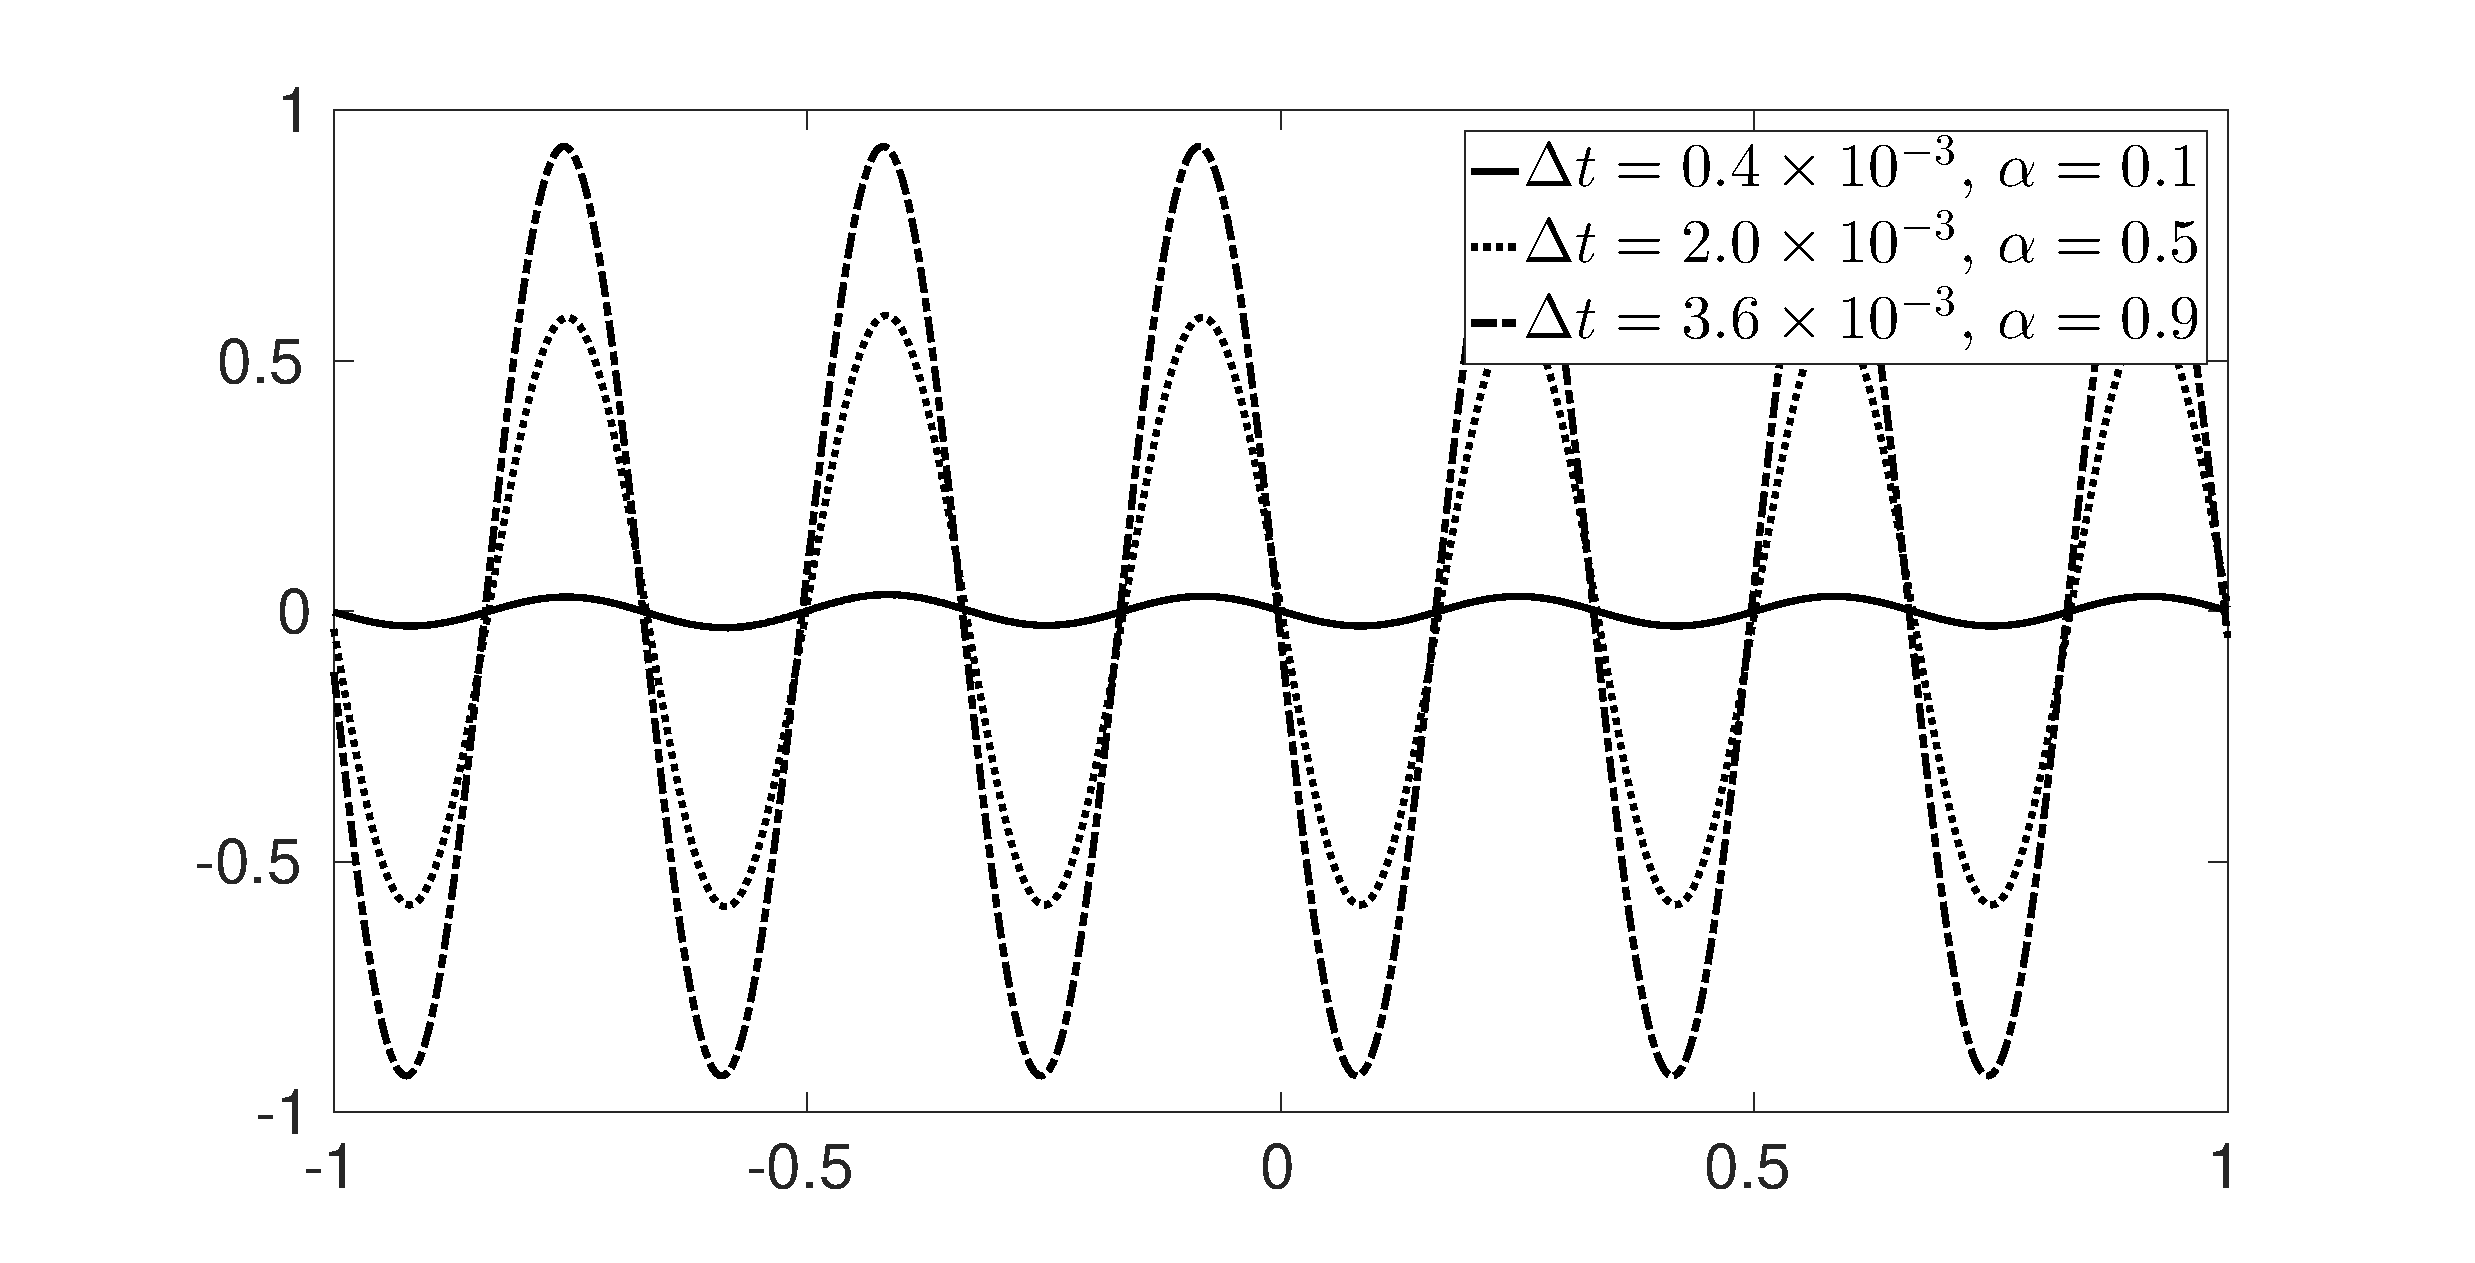
\includegraphics[width=1\textwidth]{1c.eps}
\caption{(1c) Results for different values of $\Dt$, using LF. Here we
can clearly see that the smaller value of $\Dt$, the worse the result
becomes. This is due to the fact that smaller $\Dt$ results in more
number of time steps needed to get to the same time, which in turn
means that more numerical dissipation will occur. We see that choosing
$\alpha$ as close to 1 yields the best results. }
\label{fig:1c}
\end{figure}


%\subsection{Numerical dispersion}
\begin{figure}
\centering
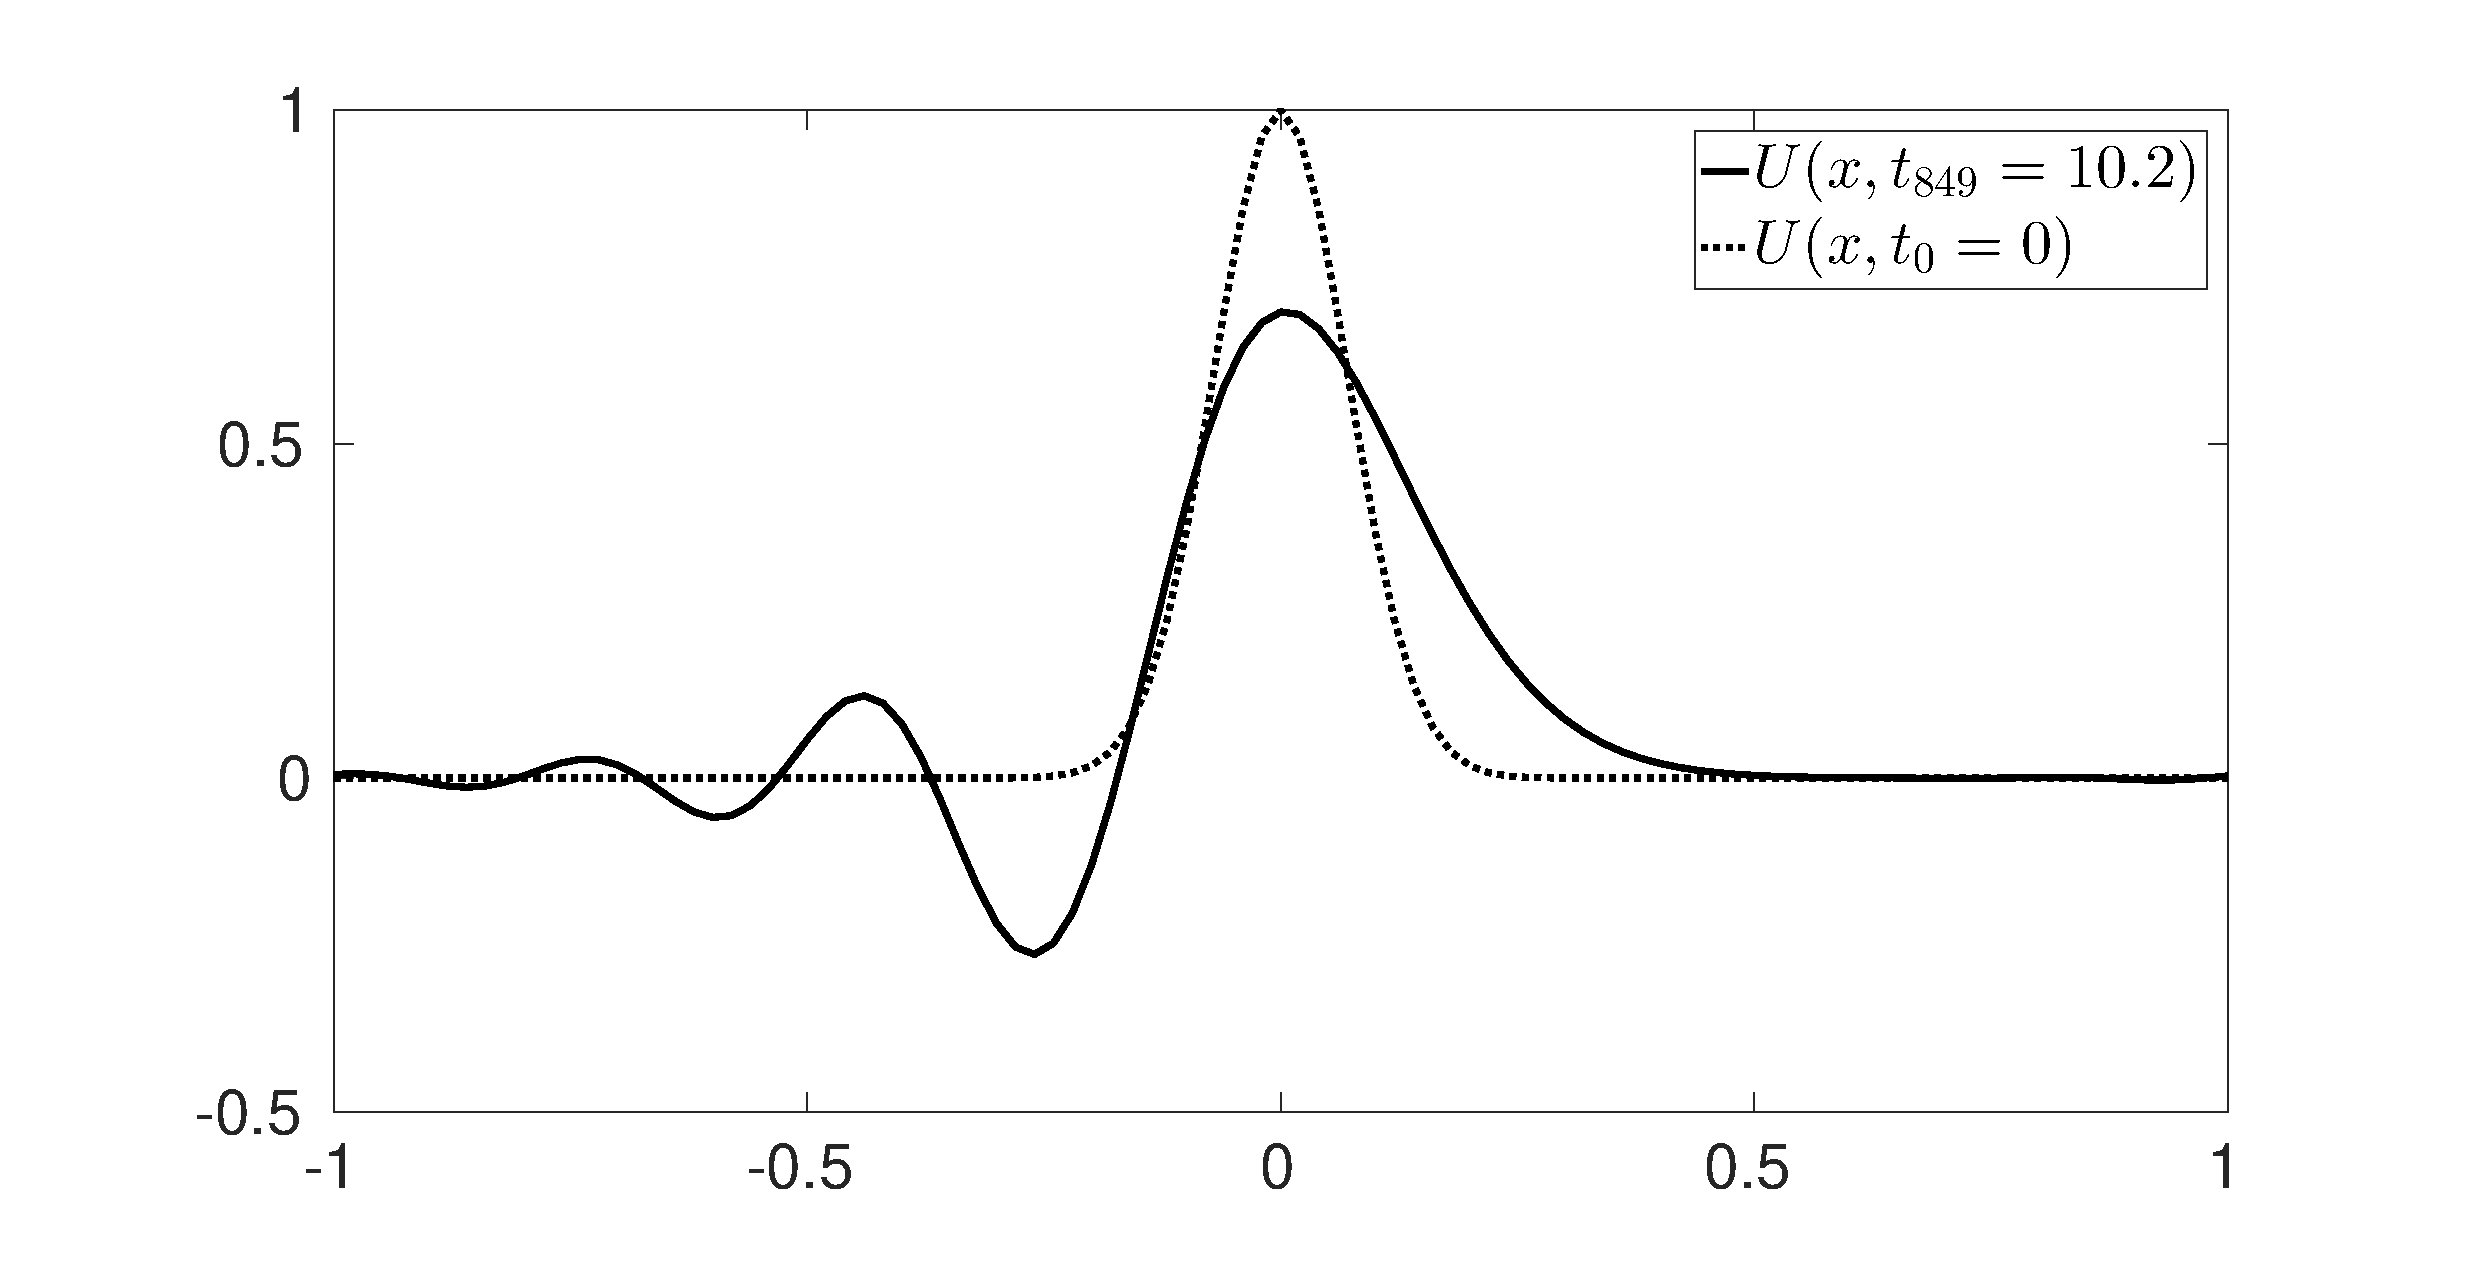
\includegraphics[width=1\textwidth]{1d.eps}
\caption{(1d) The effects of numerical dispersion on a Gaussian
  packet, using LW. We see that after time $t_N=10.2$ the Gaussian bell
  curve, consisting of many different frequencies, have been split up
  some what. The higher frequencies are lagging behind, which is seen
  as the oscillations to the left of the main peak. }
\label{fig:1d}
\end{figure}

\clearpage
\restoregeometry
\addtocounter{subsection}{4}
\subsection{Other remarks}
I personally, coming from a physics background, found the noitin of a
dispersion relation amusing. Dispersion relations are, as you might
well know, an important tool in many areas of physics espesially
involing waves of any sort (electromagnetism, quantum
mechanics, \&c.). It was therefore refreshing to see how they became a
useful tool here as well. 


\section{Stability of a scheme for the advection equation}
In this problem we have a scheme
\begin{equation}\label{eq:2_start}
\frac{(U_j^{n+1}+U_{j+1}^{n+1})-(U_j^n+U_{j+1}^n)}{2\Dt}
+a\frac{(U_{j+1}^{n+1}-U_{j}^{n+1})+(U_{j+1}^n-U_j^n)}{2\Dx}=0
\end{equation}
for the linear advection equation. And we want to show that this is
unconditionally stable.

We begin by rewriting \eqref{eq:2_start} as
\begin{equation}\label{eq:2_real_space}
(1-\alpha)U_{j}^{n+1}+(1+\alpha)U_{j+1}^{n+1}
=(1+\alpha)U_{j}^{n}+(1-\alpha)U_{j+1}^{n}.
\end{equation}
We want to show that this is stable, so what we can do is to use the
von~Neumann method. We use the Fourier transform
\begin{equation}
U_j^n=\sum_{k=0}^{J-1} A_k^n\omega_j^k
\qcomma\text{where } \omega_j^k=\exp(\ii\frac{2\pi jk}{J})=\ee^{\ii2j\theta_k},
\end{equation}
where $\theta_k=\pi k/J$. We also note that 
$U_{j+1}^m=\sum_k \ee^{\ii2\theta_k}A_k^m\omega_j^k$.

With this \eqref{eq:2_real_space} becomes
\begin{equation}
\sum_k\qty[(1-\alpha)+(1+\alpha)\ee^{\ii2\theta_k}]
A_k^{n+1}\omega_j^k
=\sum_k\qty[(1+\alpha)+(1-\alpha)\ee^{\ii2\theta_k}]
A_k^{n}\omega_j^k.
\end{equation}
Equating for all $j$ means that we can equate termwise
\begin{equation}
\qty[(1-\alpha)+(1+\alpha)\ee^{\ii2\theta_k}]A_k^{n+1}
=\qty[(1+\alpha)+(1-\alpha)\ee^{\ii2\theta_k}]A_k^{n},
\end{equation}
which gives us the amplification factor
\begin{equation}
M_k=\frac{\cancel{\ee^{\ii\theta_k}}
\qty[(1+\alpha)\ee^{-\ii\theta_k}+(1-\alpha)\ee^{\ii\theta_k}]}
{\cancel{\ee^{\ii\theta_k}}
\qty[(1-\alpha)\ee^{-\ii\theta_k}+(1+\alpha)\ee^{\ii\theta_k}]}
=\frac{\cancel{2}\qty[\cos(\theta_k)-\ii\alpha\sin(\theta_k)]}
{\cancel{2}\qty[\cos(\theta_k)+\ii\alpha\sin(\theta_k)]}.
\end{equation}
If we set $z_k=\cos(\theta_k)-\ii\alpha\sin(\theta_k)$, then
$M_k=z_k/z_k^*$ and 
\begin{equation}
\abs{M_k}=\frac{|z_k|}{|z_k^*|}=1.
\end{equation}
In other words, the absolute value of the amplification factor is
exactly 1, meaning that the amplitude of the numerical solution will
\emph{not} change. This scheme is absolute stable. \qed

\end{document}




%  LocalWords:  MFT MF Advection PDE's AMATH IC discretization MATLAB
%  LocalWords:  termwise Neumann von
